\documentclass[12pt,a4paper]{article}
\usepackage{cmap}
\usepackage[utf8]{inputenc}
\usepackage[T1,T2A]{fontenc}
\usepackage[english,russian]{babel}
\usepackage{array,booktabs,tabularx,amsmath}
\usepackage{caption,float,graphicx,qrcode}
\usepackage{geometry,hyperref,indentfirst}
\geometry{margin=25mm}
\hypersetup{unicode=true,colorlinks=true,urlcolor=blue,linkcolor=black}
\setlength{\parindent}{1.25cm}
\setlength{\parskip}{0pt}
\setlength{\emergencystretch}{2em}
\renewcommand{\labelitemi}{\textendash}
\DeclareCaptionLabelSeparator{emdash}{\space---\space}
\captionsetup[figure]{justification=centering,singlelinecheck=false,labelsep=emdash}
\addto\captionsrussian{\renewcommand{\figurename}{Рис.}}
\newcommand{\SearchRows}{%
doom & 7469 & 8112 & 0,86 & 0,61 \\
doom AND quake & 975 & 989 & 1,31 & 1,03 \\
doom OR quake & 9597 & 10271 & 1,4 & 1,11 \\
(doom OR quake) AND NOT minecraft & 9291 & 9938 & 1241,91 & 979,29 \\
NOT doom & 471364 & 470721 & 1261,57 & 1030,08 \\
games AND doom & 2697 & 4653 & 10,86 & 12,48 \\
игры AND doom & 2667 & 3703 & 13,63 & 12,76 \\
игрой AND doom & 717 & 3703 & 3,95 & 10,99 \\
(skyrim OR fallout) AND bethesda & 4425 & 4427 & 2,56 & 2,0 \\
doom AND zzzmissingterm12345 & 0 & 0 & 0,95 & 0,34 \\
}
\newcommand{\SearchSurfaceMiB}{4,59}
\newcommand{\SearchLemmaMiB}{163,47}
\newcommand{\SearchRepeats}{3}

\begin{document}
\hypersetup{pageanchor=false}
\begin{titlepage}
\begin{center}
{\large МОСКОВСКИЙ АВИАЦИОННЫЙ ИНСТИТУТ\\
(НАЦИОНАЛЬНЫЙ ИССЛЕДОВАТЕЛЬСКИЙ УНИВЕРСИТЕТ)}
\vspace{18pt}
{\large Факультет информационных технологий и прикладной математики}

{\large Кафедра вычислительной математики и~программирования}
\vfill
{\large\textbf{Лабораторная работа №8 по курсу\\ «Информационный поиск»}}
\vspace{12mm}

{\large\textbf{Булев поиск}}
\vfill
\begin{flushright}
\begin{tabular}{@{}r@{:\hspace{0.6em}}l@{}}
\textit{Студент} & К.\,А. Арусланов\\
\textit{Группа} & М8О-403Б-23\\
\textit{Преподаватель} & А.\,А. Кухтичев\\
\textit{Дата} & 07.11.2026\\
\textit{Оценка} &
\end{tabular}
\end{flushright}
\vfill
Москва, 2026
\end{center}
\end{titlepage}
\hypersetup{pageanchor=true}
\setcounter{page}{2}
\tableofcontents
\newpage

\section{Постановка задачи}
Реализовать булев поиск по инвертированному индексу корпуса.
Поддержать конъюнкцию, дизъюнкцию, отрицание, приоритет операций
и группировку скобками. Поисковую логику и структуры данных
реализовать самостоятельно на C++. Предусмотреть консольную утилиту,
читающую запросы из стандартного ввода, и веб-форму с HTML-выдачей.

\section{Метод решения}
\subsection{Множества документов и язык запросов}
Используется индекс ЛР7, построенный по фиксированному снимку
478\,833 публикаций об играх из восьми русскоязычных и англоязычных
источников. Индексированы заголовки и основные тексты.
Исходный корпус при поиске не читается; заголовки, источники и URL
извлекаются из таблицы метаданных индекса.

Пусть $U$ --- множество ID всех документов, а $L(t)$ --- упорядоченный
список документов, содержащих термин $t$. Тогда
\[
R(A\mathbin{\mathrm{AND}}B)=R(A)\cap R(B),\qquad
R(A\mathbin{\mathrm{OR}}B)=R(A)\cup R(B),
\]
\[
R(\mathrm{NOT}\ A)=U\setminus R(A).
\]
Множество $U$ включает документы без токенов. ID являются
64-битными числами и могут иметь пропуски: дополнение строится
по таблице документов, а не по числовому диапазону ID.

Приоритет операций: \texttt{NOT}, затем \texttt{AND}, затем \texttt{OR}.
Скобки меняют порядок вычислений. Допускаются символьные аналоги
\texttt{!}, \texttt{\&}, \texttt{|}. Между словами требуется явная операция.
Например, \texttt{doom OR quake AND NOT minecraft} означает
\texttt{doom OR (quake AND (NOT minecraft))}.

\subsection{Разбор и потоковое вычисление}
Рекурсивный спуск строит собственное дерево выражения.
Каждый лист обращается к дисковому словарю и открывает независимый
курсор списка документов. Внутренний узел хранит текущие ID
дочерних потоков и последовательно выполняет операцию над ними.

При пересечении продвигается поток с меньшим ID; совпавший ID выдаётся
один раз. При объединении выдаётся меньший ID, а совпадение продвигает
оба потока. Разность пропускает ID левого потока, присутствующие в правом.
Поэтому порядок и уникальность сохраняются на каждом уровне дерева.
Промежуточные множества и полная выдача в памяти не сохраняются.

Операция над двумя отсортированными списками длины $p$ и $q$ требует
$O(p+q)$ шагов в худшем случае. Память определяется деревом,
текущими элементами потоков, файловыми буферами и словарём лемматизации,
а не общим числом найденных документов. Запрос ограничен 8192 байтами,
64 операндами и 64 уровнями вложенности; после раскрытия лемм
допускается не более 1024 узлов. Превышение возвращает явную ошибку.

\subsection{Словоформы и леммы}
Операнды нормализуются тем же токенизатором, что и документы.
Режим словоформ обращается к исходному пространству терминов.
В режиме лемм каждый операнд разбирается словарём из ЛР4,
а списки всех его различных лемм объединяются.
Таким образом, для множества разборов $M(w)$
\[
L_{\mathrm{query}}(w)=\bigcup_{\ell\in M(w)}L_{\mathrm{lemma}}(\ell).
\]
Это соответствует политике построения индекса: документ включён
в список каждой допустимой леммы его слов. Неизвестные слова сохраняются.
Например, отрицание \texttt{NOT стали} исключает документы из объединения
списков «сталь» и «стать». Контекстное снятие неоднозначности отсутствует.
Совпадение словаря запроса со словарём индекса проверяется
по сохранённому 64-битному отпечатку файла.

\subsection{Интерфейсы}
Консольная утилита принимает по одному UTF-8-запросу в строке
стандартного ввода и выдаёт по одному JSON-объекту в строке
стандартного вывода. Для каждого запроса возвращаются точное число
совпадений, время вычисления и ограниченный список документов
с ID, заголовками, URL и источниками.
Ошибка одной строки не препятствует обработке следующих.

Веб-форма предоставляет ввод выражения и переключение режима.
Выдача содержит число совпадений и первые 20 заголовков со ссылками.
Python передаёт запрос C++-процессу через UTF-8 stdin и преобразует
полученные метаданные в HTML; поисковых структур в Python нет.
Для каждого обращения формы запускается отдельный процесс,
поэтому время HTTP-ответа дополнительно включает загрузку словаря.

Оба интерфейса упорядочивают результаты по ID, без ранжирования.
Ограничение размера отображаемой выдачи не прекращает вычисление:
для точного числа совпадений поток ID читается до конца.

\section{План и результаты тестирования}
На контрольном корпусе проверяются приоритеты, скобки, повторные
операнды, тождества множеств, законы де Моргана и двойное отрицание.
Для 64 автоматически составленных выражений в каждом из двух режимов
результаты сравниваются с независимой таблицей истинности для всех
сочетаний трёх терминов. Используются термины, одинаково представленные
в обоих пространствах; преобразование словоформ в леммы проверяется отдельно.
В корпус включены пустой документ и произвольные 64-битные ID.

Отдельно проверяются нормализация, оба пространства терминов,
неоднозначные леммы, неизвестные слова и несовпадающий словарь.
Проверки CLI охватывают точное число совпадений при ограниченной выдаче,
корректность JSON, экранирование метаданных, UTF-8, CRLF,
последнюю строку без перевода строки и продолжение после ошибки.
Некорректные выражения и превышения ограничений отклоняются.

Успешно пройдены 11 GoogleTest и одна процессная проверка CLI.
Три Python-теста проверяют передачу UTF-8 в нативную программу,
HTTP-форму, обработку ошибок и экранирование HTML.
Журнал с отдельными тест-кейсами приложен в \path{lab8/tests.txt}.
Команды пересборки и прямого запуска GoogleTest приведены
в \path{doc/lab8_run.md}.

\section{Результаты на корпусе}
\subsection{Число совпадений и время}
В таблице приведены точные размеры множеств и медианы
\SearchRepeats{} повторений каждого запроса в одном процессе
для каждого режима. Измерено время нормализации, разбора выражения
и полного получения потока ID. Загрузка словаря, чтение метаданных
и вывод JSON в это время не включены. Применена нативная Windows
Release-сборка GCC 13.1.0; файловый кеш между повторениями не очищался.

\begin{table}[H]
\centering
\small
\begin{tabularx}{\linewidth}{@{}Xrrrr@{}}
\toprule
 & \multicolumn{2}{c}{Документы} & \multicolumn{2}{c}{Время, мс}\\
Запрос & Формы & Леммы & Формы & Леммы\\
\midrule
\SearchRows
\bottomrule
\end{tabularx}
\end{table}

Для \texttt{doom} исходное число совпадений 7469 совпадает
с документной частотой из ЛР7. Пересечение с \texttt{quake}
уменьшает множество до 975 документов, объединение увеличивает
его до 9597. Отрицание \texttt{NOT doom} возвращает
$478833-7469=471364$ документа. Пересечение с отсутствующим
термином пусто в обоих режимах.

Запросы «игры AND doom» и «игрой AND doom» дают различные
множества словоформ: 2667 и 717 документов. После лемматизации
обе формы приводят к одному результату из 3703 документов.
Это демонстрирует устранение различий между падежными формами.
Увеличение количества кандидатов само по себе не доказывает
рост точности или полноты относительно информационной потребности:
для такой оценки необходима отдельная разметка релевантности.

\subsection{Память и ограничения производительности}
Пиковый рабочий набор поискового процесса составил
\SearchSurfaceMiB{} МиБ для словоформ и \SearchLemmaMiB{} МиБ
для лемм. Разница определяется главным образом загруженным
морфологическим словарём. Индекс размером около 1,72 ГБ
целиком в память не загружался. Измерен рабочий набор процесса,
без системного файлового кеша.

Отрицание перечисляет множество документов, поэтому запросы
с \texttt{NOT} существенно медленнее простых объединений
и пересечений. В текущем дереве выражение \texttt{A AND NOT B}
вычисляет поток $U\setminus B$ и пересекает его с $A$.
Преобразование в непосредственную разность $A\setminus B$
позволило бы избежать полного перечисления $U$.
Планирование по документным частотам и прыжки по спискам
также могут уменьшить число чтений; в данной работе
они не применяются.

\subsection{Пример веб-поиска}
На рис.~\ref{fig:boolean-web} показано выполнение запроса
«покупка AND студии AND bungie» в пространстве словоформ.
Найдены 22 документа. Условие требует наличия всех трёх слов
в индексируемых полях документа; их соседство и порядок
не проверяются. Поэтому совпадение может находиться в основном
тексте и не быть полностью представлено в заголовке выдачи.

\begin{figure}[H]
\centering
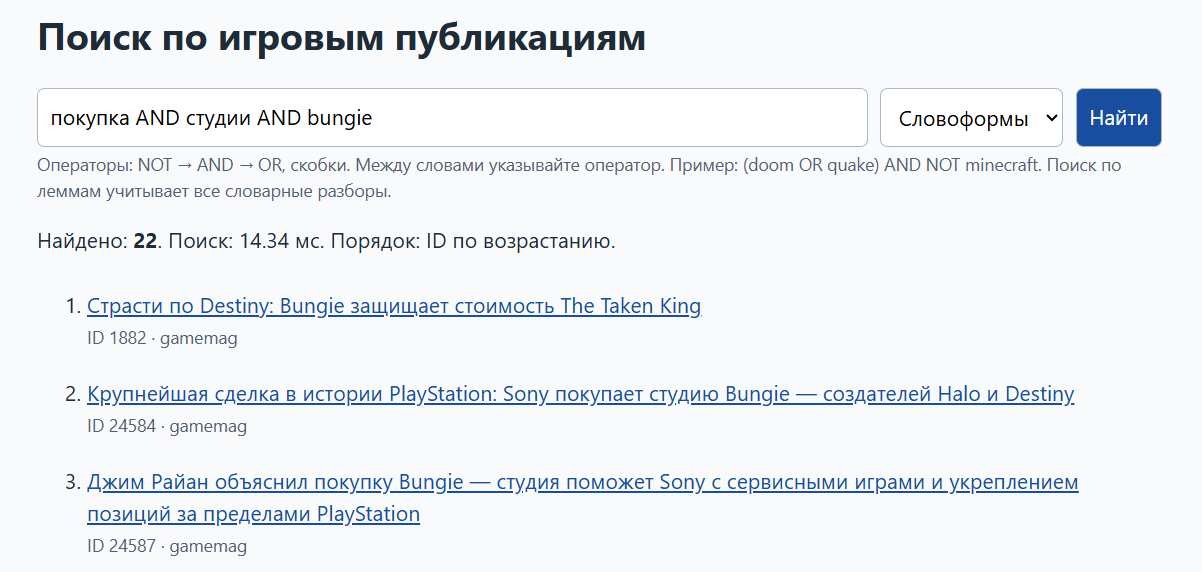
\includegraphics[width=\linewidth]{img/bungie_sony.png}
\caption{Булев запрос с тремя условиями AND в веб-интерфейсе}
\label{fig:boolean-web}
\end{figure}

\subsection{Воспроизводимость}
Скрипт \path{run_lab8.py} запускает тесты и пакет запросов
из \path{tests/fixtures/lab8_queries.txt}.
Сохранены исходные JSONL-ответы, первые ID и метаданные,
времена повторений, измерения памяти и отпечатки входных файлов.
Результаты находятся в \path{doc/lab8/}.
Исходный индекс открывается только для чтения.

Исходный код:
\href{https://github.com/kirbasss/MAI-IR/tree/lab8}{github.com/kirbasss/MAI-IR/tree/lab8}.
\begin{figure}[H]
\centering
\begingroup
\hypersetup{urlcolor=black}
\qrcode[height=28mm]{https://github.com/kirbasss/MAI-IR/tree/lab8}
\endgroup
\caption{Ссылка на ветку лабораторной работы №8}
\end{figure}

\section{Вывод}
Реализованы разбор булевых выражений и потоковое вычисление
точных множеств документов по сохранённому индексу.
Поддержаны словоформы, леммы и согласованное раскрытие
морфологической неоднозначности. Консольная утилита и веб-форма
используют одно поисковое ядро C++.

Проверки подтверждают соответствие выдачи булевой алгебре,
в том числе для пустых документов, неизвестных терминов
и произвольных ID. Поиск испытан на 478\,833 документах;
работа на миллионном корпусе этими измерениями не проверялась.
Основные ограничения --- полное перечисление корпуса при отрицании,
отсутствие ранжирования, координат слов и контекстного снятия омонимии.
Дальнейшие направления: планирование выражений, прыжки по спискам,
цитатный поиск и оценка релевантности на размеченных запросах.
\end{document}
